\section{Introduction}

In robotics, some tasks are relatively easy to perform with complete knowledge 
of the environment, but become more challenging when the environment is only 
partially observable using a robot's sensors. Imitation learning deals with 
this problem by recording the trajectories of an omniscient controller 
performing the desired task, then training a machine learning model to 
replicate them using just the data from the sensors. As such, the machine 
learning model must learn how to extract the relevant information from the data 
it receives, sidestepping the difficulty of implementing the perception part 
manually.

The target platform we choose for our project is the 
marXbot~\cite{bonani2010marxbot}, a research robot originally designed to study 
collective and swarm robotics. The main characteristic making the marXbot 
interesting for this project is its rotating laser scanner, which perceives 
distances and colours of the objects surrounding the robot.

The experiments are run in Enki~\cite{enki}, a high-performance open-source 
simulator for planar robots, which provides collision detection and limited 
physics support for robots evolving on a flat surface. Moreover, it can 
simulate groups of robots hundreds of times faster than real-time.

\begin{figure}[htbp]
	\centerline{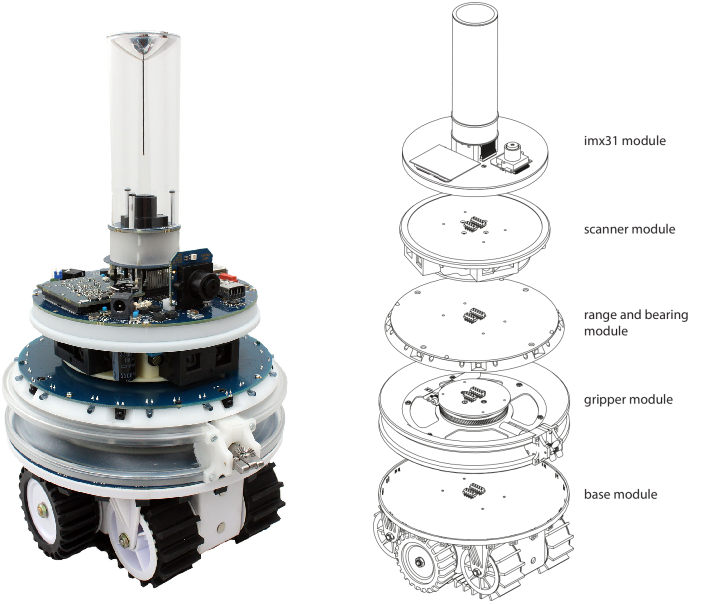
\includegraphics[width=.8\columnwidth]{introduction/marxbot}}
	\caption{Actual image and exploded CAD view of a marXbot.}
	\label{fig:marxbot}
\end{figure}

The task that we 

%The main objective of this project is learning to perform specific 
%interactions between the robot and objects in the 
%environment.
%Write an omniscient controller that performs the desired interaction with 
%complete knowledge of the environment (e.g. 
%position the robot at a certain location relative to an object) using Enki.
%Generate a dataset of simulation runs through Enki. 
%Through imitation learning, train an end-to-end neural network that receives 
%as inputs the sensor distances and the 
%camera image readings and produces commands for the motors that are the left 
%and the right wheel target speeds.
%Evaluate the model trained using Enki.
% 
